\documentclass[12pt,a4paper]{article}
\usepackage[a4paper,margin=1in]{geometry}
\usepackage{graphicx}
\usepackage{booktabs}
\usepackage{amsmath,amssymb}
\usepackage{float}
\usepackage{hyperref}
\usepackage{xcolor}
\usepackage{listings}
\usepackage{enumitem}
\usepackage{fancyhdr}
\usepackage{longtable}
\hypersetup{colorlinks=true,linkcolor=blue,urlcolor=blue}
\pagestyle{fancy}
\fancyhf{}
\lhead{ICS1512}
\rhead{Machine Learning Algorithms Laboratory}
\cfoot{\thepage}
\lstset{
language=Python,
basicstyle=\ttfamily\small,
numbers=left,
frame=single,
breaklines=true,
showstringspaces=false
}
\begin{document}
\begin{tabular}{|p{4cm}|p{11cm}|}
\hline
Experiment No. & 6\\ \hline
Experiment Title & Ensemble Learning: Bagging, AdaBoost, Gradient Boosting and Stacking -- A Comparative Classification Study\\ \hline
GitHub Repository & \url{https://github.com/Dharika-2006/ML-LAB-ASSIGMENTS} \\ \hline
Student Name & Dharika Shree K\\ \hline
Register Number & 3122247001014\\ \hline
Faculty & Dr. Poreddy Ajay Kumar Reddy \\ \hline
Submission Date & 30.08.2026\\ \hline
\end{tabular}
\section{Objective}
To build and compare four ensemble-based classifiers -- Bagging, AdaBoost, Gradient Boosting, and Stacking -- on the Wisconsin Diagnostic Breast Cancer dataset, tune their hyperparameters using 5-Fold Cross-Validation via GridSearchCV, and evaluate them using accuracy, precision, recall, F1-score, confusion matrices, and ROC curves with AUC.

\section{Problem Statement}
\textbf{Problem:} Classify breast cancer tumors as malignant or benign using four different ensemble learning strategies -- Bagging, AdaBoost, Gradient Boosting, and Stacking -- and compare their performance on the Wisconsin Diagnostic Breast Cancer dataset by tuning hyperparameters using 5-Fold Cross-Validation and evaluating them using accuracy, precision, recall, F1-score, confusion matrices, and ROC curves.

\textbf{Input:} The Wisconsin Diagnostic Breast Cancer dataset, containing 569 samples with 30 numerical features describing characteristics of breast cell nuclei, with each sample classified as malignant or benign.

\textbf{Output:} Trained and tuned Bagging, AdaBoost, Gradient Boosting, and Stacking models, hyperparameter tuning results, confusion matrices, ROC curves, and a final accuracy/precision/recall/F1-score comparison across all four algorithms, with identification of the best-performing model.

\section{Dataset Description}
\begin{longtable}{|p{6cm}|p{8cm}|}
\hline
Dataset Name & Wisconsin Diagnostic Breast Cancer Dataset\\ \hline
Dataset Source & Scikit-learn (\texttt{load\_breast\_cancer})\\ \hline
Number of Samples & 569\\ \hline
Number of Features & 30 \\ \hline
Number of Classes & 2 \\ \hline
Missing Values & None \\ \hline
Train-Test Split & 80\% training and 20\% testing (stratified)\\ \hline
\end{longtable}

\section{Exploratory Data Analysis}
\begin{itemize}
\item Dataset overview
\item Statistical summary
\item Missing value analysis
\item Class distribution
\end{itemize}

\subsection*{Figure: Dataset Overview}
\begin{figure}[H]
\centering
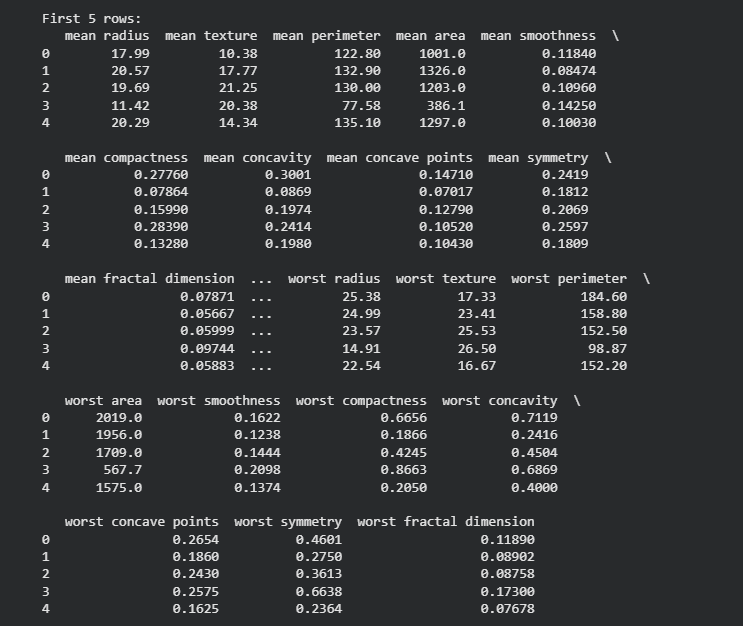
\includegraphics[width=0.9\linewidth]{overview.png}
\caption{First five rows of the feature set showing sample values across the 30 numerical columns}
\end{figure}
\textbf{Inference:}
The dataset consists of 569 samples and 30 continuous numerical features, all stored as \texttt{float64}, covering measurements such as radius, texture, perimeter, area, smoothness, compactness, concavity, concave points, symmetry, and fractal dimension, each summarized as a mean, standard error, and worst value. No categorical variables are present, so no encoding is required for the input features. The consistent scale differences visible across columns (e.g., area values in the hundreds versus smoothness values below 1) suggested that feature scaling would be necessary for distance- or margin-based models such as SVM. This overview confirmed that the dataset was clean and ready for direct use in the ensemble pipelines.

\subsection*{Figure: Missing Value and Class Distribution Check}
\begin{figure}[H]
\centering
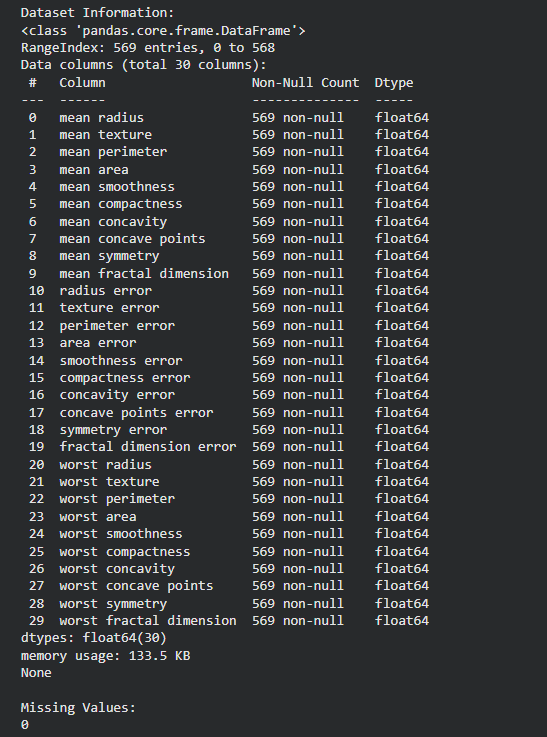
\includegraphics[width=0.9\linewidth]{info.png}
\caption{Dataset information summary and missing value count}
\end{figure}
\textbf{Inference:}
The \texttt{DataFrame.info()} output confirmed that all 30 columns contain 569 non-null \texttt{float64} entries, and the total missing-value count returned by \texttt{isnull().sum().sum()} was 0. This meant no imputation or row/column removal was needed before modelling. The dataset's memory footprint (approximately 133.5 KB) also confirmed it was small enough to allow exhaustive grid search across all four ensemble models without computational bottlenecks.

\subsection*{Figure: Class Distribution}
\begin{figure}[H]
\centering

\includegraphics[width=0.6\linewidth]{cld1.png}
\caption{Class distribution of benign and malignant samples}
\end{figure}
\textbf{Inference:}
The dataset contains 357 benign samples (approximately 62.7\%) and 212 malignant samples (approximately 37.3\%). Thus, the classes are not perfectly balanced, although the imbalance is not extreme. Since both classes have a substantial number of samples, the dataset is suitable for binary classification. The train-test split was stratified to preserve approximately the same class distribution in both the training and testing sets. Therefore, accuracy alone may not provide the complete picture, making precision, recall, and F1-score useful additional evaluation metrics for comparing the four ensemble models.

\section{Data Preprocessing}
\begin{itemize}
\item \textbf{Missing value handling:} No missing value handling was performed, as the dataset contains 0 missing values, verified using \texttt{X.isnull().sum().sum()}.

\item \textbf{Encoding:} Not required -- the 30 input features were already numerical, and the target variable was already encoded as 0 (malignant) and 1 (benign) by \texttt{load\_breast\_cancer}.

\item \textbf{Feature scaling:} \texttt{StandardScaler} was applied only within the SVM pipeline, since SVM is a margin-based model sensitive to feature magnitude. The tree-based components of Bagging, AdaBoost, and Gradient Boosting did not require scaling.

\item \textbf{Train-test split:} The dataset was divided into 80\% training and 20\% testing sets using \texttt{train\_test\_split}, with \texttt{test\_size=0.20}, \texttt{stratify=y}, and \texttt{random\_state=42}. This produced 455 training samples and 114 testing samples while preserving the class distribution.

\item \textbf{Feature engineering:} None -- the original 30 numerical features were used directly for model training.
\end{itemize}

\section{Machine Learning Algorithm}

\subsection*{Bagging Classifier}
\textbf{Working principle:} Bagging (Bootstrap Aggregating) trains multiple Decision Tree base estimators independently, each on a different bootstrap sample (random sample with replacement) of the training data, and aggregates their predictions through majority voting.

\textbf{Mathematical formulation:}
\[
\hat{y} = \operatorname{mode}\{h_1(x), h_2(x), \ldots, h_B(x)\}
\]
where $h_b(x)$ is the prediction of the $b$-th base learner trained on a bootstrap sample, and $B$ is the total number of estimators.

\textbf{Advantages:} Reduces variance and overfitting, works well with high-variance base learners such as decision trees, and is easily parallelizable.

\textbf{Limitations:} Does not reduce bias; provides limited benefit when the base learner already has low variance.

\subsection*{AdaBoost Classifier}
\textbf{Working principle:} AdaBoost sequentially trains weak learners (decision stumps with \texttt{max\_depth=1}), where each subsequent learner focuses more on samples misclassified by earlier learners through adaptive re-weighting of the training samples.

\textbf{Mathematical formulation:}
\[
H(x) = \operatorname{sign}\left(\sum_{t=1}^{T}\alpha_t h_t(x)\right), \quad \alpha_t = \frac{1}{2}\ln\left(\frac{1-\epsilon_t}{\epsilon_t}\right)
\]
where $\epsilon_t$ is the weighted classification error of the $t$-th weak learner.

\textbf{Advantages:} Reduces both bias and variance, and often achieves high accuracy even with very simple base learners.

\textbf{Limitations:} Sensitive to noisy data and outliers, since misclassified samples are given progressively higher weight.

\subsection*{Gradient Boosting Classifier}
\textbf{Working principle:} Gradient Boosting builds an additive ensemble of decision trees sequentially, where each new tree is trained to fit the negative gradient (residual error) of the loss function with respect to the current ensemble's predictions.

\textbf{Mathematical formulation:}
\[
F_m(x) = F_{m-1}(x) + \gamma_m h_m(x)
\]
where $h_m$ is trained on the pseudo-residuals $-\left[\dfrac{\partial L(y,F(x))}{\partial F(x)}\right]_{F=F_{m-1}}$.

\textbf{Advantages:} Typically achieves very high predictive accuracy and can model complex non-linear relationships through flexible loss functions.

\textbf{Limitations:} Prone to overfitting if not regularized properly, sequential training limits parallelization, and performance is sensitive to hyperparameters such as learning rate and tree depth.

\subsection*{Stacking Classifier}
\textbf{Working principle:} Stacking combines predictions from multiple diverse base learners (SVM, Gaussian Naive Bayes, and Decision Tree) using a meta-learner (Logistic Regression) trained on the cross-validated out-of-fold predictions of the base learners.

\textbf{Mathematical formulation:}
\[
\hat{y} = g\big(h_1(x), h_2(x), h_3(x)\big)
\]
where $h_1, h_2, h_3$ are the base learners' predictions and $g$ is the meta-learner.

\textbf{Advantages:} Leverages the complementary strengths of structurally different algorithms, often outperforming any individual base model.

\textbf{Limitations:} Higher computational cost and complexity, and risk of meta-learner overfitting if cross-validation is not used correctly (mitigated here with \texttt{cv=5}).

\section{Experimental Setup}
\begin{tabular}{ll}
\toprule
Python Version & Python 3 (Google Colab runtime)\\
Scikit-Learn Version & As installed in the Google Colab environment\\
IDE & Google Colaboratory (Jupyter-based notebook)\\
Operating System & Linux (Google Colab backend)\\
Hardware & Google Colab-provided CPU runtime\\
\bottomrule
\end{tabular}

\section{Hyperparameter Selection}
\begin{tabular}{ll}
\toprule
Parameter & Value\\
\midrule
Train-Test Split & 80:20, stratified, \texttt{random\_state=42}\\
Cross-Validation & 5-fold, scoring = accuracy\\
Bagging -- search space & \texttt{n\_estimators} $\in\{10,50,100\}$,\\
& \texttt{max\_samples} $\in\{0.5,0.8,1.0\}$,\\
& \texttt{max\_features} $\in\{0.5,0.8,1.0\}$\\
Bagging -- best params & \texttt{n\_estimators=100}, \texttt{max\_samples=0.8},\\
& \texttt{max\_features=0.5}\\
Bagging -- best CV Accuracy & 0.9604\\
AdaBoost -- search space & \texttt{n\_estimators} $\in\{50,100,150\}$,\\
& \texttt{learning\_rate} $\in\{0.01,0.1,1.0\}$\\
AdaBoost -- best params & \texttt{n\_estimators=100}, \texttt{learning\_rate=1.0}\\
AdaBoost -- best CV Accuracy & 0.9736\\
Gradient Boosting -- search space & \texttt{n\_estimators} $\in\{50,100,150\}$,\\
& \texttt{learning\_rate} $\in\{0.01,0.1,0.2\}$,\\
& \texttt{max\_depth} $\in\{1,2,3\}$\\
Gradient Boosting -- best params & \texttt{n\_estimators=100}, \texttt{learning\_rate=0.2},\\
& \texttt{max\_depth=1}\\
Gradient Boosting -- best CV Accuracy & 0.9802\\
Stacking -- base models & SVM (with StandardScaler), Gaussian Naive Bayes,\\
& Decision Tree\\
Stacking -- meta-learner & Logistic Regression (\texttt{max\_iter=1000})\\
Stacking -- cv & 5\\
\bottomrule
\end{tabular}

\section{Results}
\begin{longtable}{lcccc}
\toprule
Model & Accuracy & Precision & Recall & F1-score\\
\midrule
Bagging & 0.9474 & 0.9583 & 0.9583 & 0.9583\\
AdaBoost & 0.9561 & 0.9467 & 0.9861 & 0.9660\\
Gradient Boosting & 0.9649 & 0.9595 & 0.9861 & 0.9726\\
Stacking & 0.9737 & 0.9726 & 0.9861 & 0.9793\\
\bottomrule
\end{longtable}

\noindent The tuned Stacking classifier clearly outperforms the other three ensembles, achieving 97.37\% accuracy compared to 96.49\% for Gradient Boosting, 95.61\% for AdaBoost, and 94.74\% for Bagging. Stacking also achieves the highest precision (97.26\%) and shares the highest recall (98.61\%) with AdaBoost and Gradient Boosting, resulting in the best overall F1-score (97.93\%). Bagging, while still strong, performed the weakest of the four, consistent with its primary strength being variance reduction rather than bias reduction. Overall, combining diverse base learners through stacking provided better classification performance and stability than any single boosting or bagging strategy on this dataset.

\section{Result Visualization}
Include all graphs generated during the experiment.

\subsection*{1. Class Distribution}
See Section 4 -- the dataset contains 357 benign samples (62.7\%) and 212 malignant samples (37.3\%). The classes are therefore moderately imbalanced, making stratified train-test splitting and metrics such as precision, recall, and F1-score useful for evaluation.

\subsection*{2. Confusion Matrix}

\begin{figure}[H]
\centering
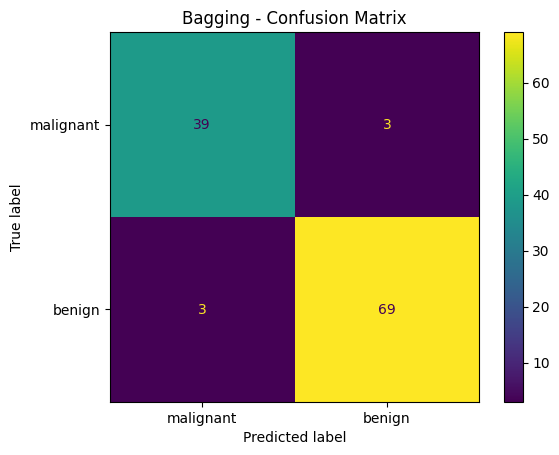
\includegraphics[width=0.55\linewidth]{conf_bagging.png}
\caption{Confusion Matrix -- Bagging}
\end{figure}

\begin{figure}[H]
\centering
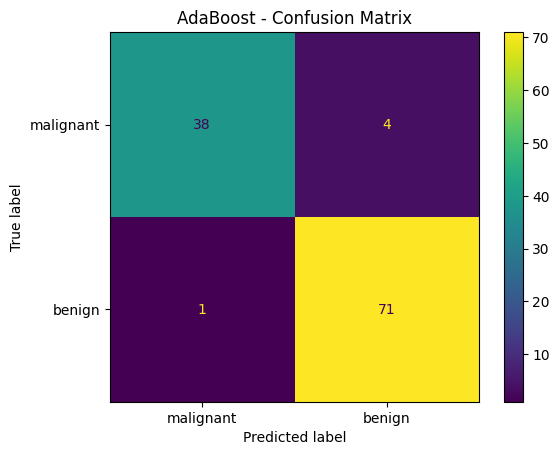
\includegraphics[width=0.55\linewidth]{conf_ada.png}
\caption{Confusion Matrix -- AdaBoost}
\end{figure}

\begin{figure}[H]
\centering
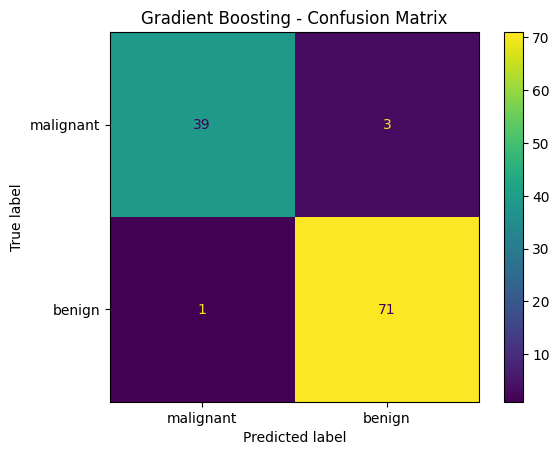
\includegraphics[width=0.55\linewidth]{conf_gb.png}
\caption{Confusion Matrix -- Gradient Boosting}
\end{figure}

\begin{figure}[H]
\centering
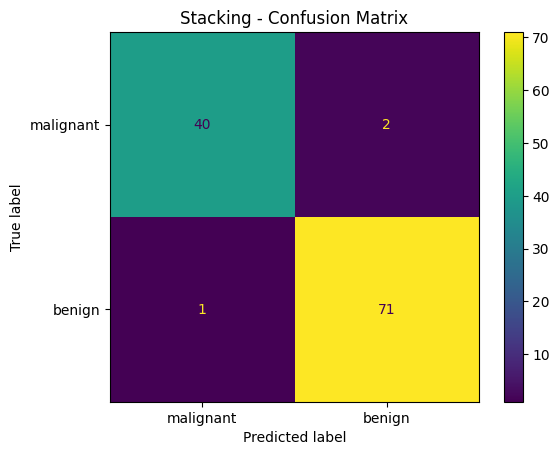
\includegraphics[width=0.55\linewidth]{conf_stack.png}
\caption{Confusion Matrix -- Stacking}
\end{figure}

\textbf{Inference:}
Bagging produced 6 misclassifications (3 false positives, 3 false negatives). AdaBoost produced 5 misclassifications (4 false positives, 1 false negative). Gradient Boosting also produced 4 misclassifications (3 false positives, 1 false negative). Stacking produced the fewest errors overall, with only 3 misclassifications (2 false positives, 1 false negative). This confirms that Stacking not only achieves the highest accuracy but also minimizes both false positives and false negatives most effectively among the four models, which is particularly important in a diagnostic setting where false negatives are costly.

\subsection*{3. ROC Curve}

\begin{figure}[H]
\centering

\includegraphics[width=0.75\linewidth]{roc.png}
\caption{ROC Curve Comparison -- Bagging, AdaBoost, Gradient Boosting, and Stacking}
\end{figure}

\textbf{Inference:}
The ROC curves illustrate the trade-off between the true positive rate and false positive rate for all four ensemble classifiers. Stacking is expected to show the strongest overall discrimination, consistent with its highest test accuracy, precision, and F1-score, followed closely by Gradient Boosting. Bagging is expected to show the weakest ROC performance among the four, aligning with its comparatively lower test accuracy. The AUC values for each curve provide an additional measure of how well each model separates the malignant and benign classes across all classification thresholds.

\subsection*{4. Model Comparison}

\begin{figure}[H]
\centering

\includegraphics[width=0.7\linewidth]{comp.png}
\caption{Performance comparison of Bagging, AdaBoost, Gradient Boosting, and Stacking across Accuracy, Precision, Recall, and F1-score}
\end{figure}

\textbf{Inference:}
The bar chart comparison shows a clear performance ordering: Stacking $>$ Gradient Boosting $>$ AdaBoost $>$ Bagging, in terms of accuracy and F1-score. All four models achieve recall above 0.95, indicating that each ensemble strategy is reasonably reliable at identifying malignant cases. The gap between Bagging and the other three methods is the most noticeable, suggesting that on this dataset, bias-reduction strategies (boosting, stacking) generalize better than a purely variance-reduction strategy (bagging).

\section{Discussion}
All four ensemble methods performed well on the Wisconsin Diagnostic Breast Cancer dataset, with test accuracies ranging from 94.74\% (Bagging) to 97.37\% (Stacking). Stacking, which combines SVM, Naive Bayes, and Decision Tree base learners through a Logistic Regression meta-learner, achieved the best overall performance across accuracy, precision, and F1-score, while sharing the top recall value with AdaBoost and Gradient Boosting. Interestingly, Gradient Boosting achieved the highest cross-validation accuracy during hyperparameter tuning (0.9802), even though its final test accuracy (0.9649) was slightly lower than Stacking's, suggesting that combining diverse algorithms generalizes marginally better to unseen data than boosting a single type of weak learner. Bagging consistently performed the weakest of the four, which is expected since its main strength lies in variance reduction rather than bias reduction. All models achieved high recall, which is clinically important since false negatives are more costly than false positives in cancer diagnosis. A limitation of this experiment is that all four models were compared using a single train-test split rather than nested cross-validation, which could be explored in future work for a more robust comparison.

\section{Conclusion}
This experiment implemented and compared four ensemble learning techniques -- Bagging, AdaBoost, Gradient Boosting, and Stacking -- on the Wisconsin Diagnostic Breast Cancer dataset. After hyperparameter tuning using 5-fold cross-validation, the Stacking ensemble achieved the best test performance, with 97.37\% accuracy, 97.26\% precision, 98.61\% recall, and a 97.93\% F1-score, outperforming Gradient Boosting (96.49\%), AdaBoost (95.61\%), and Bagging (94.74\%). The results demonstrate that combining diverse, complementary base learners through stacking provides better and more stable classification performance than individual bagging or boosting strategies on this dataset.

\section{References}
\begin{enumerate}
\item Scikit-learn developers, Ensemble methods, scikit-learn documentation: \url{https://scikit-learn.org/stable/modules/ensemble.html}

\item Breiman, L., "Bagging predictors," \textit{Machine Learning}, vol. 24, no. 2, pp. 123--140, 1996.

\item Freund, Y. and Schapire, R. E., "A decision-theoretic generalization of on-line learning and an application to boosting," \textit{Journal of Computer and System Sciences}, vol. 55, no. 1, pp. 119--139, 1997.

\item Friedman, J. H., "Greedy function approximation: A gradient boosting machine," \textit{Annals of Statistics}, vol. 29, no. 5, pp. 1189--1232, 2001.

\item Wolpert, D. H., "Stacked generalization," \textit{Neural Networks}, vol. 5, no. 2, pp. 241--259, 1992.

\item UCI Machine Learning Repository, Wisconsin Diagnostic Breast Cancer Dataset: \url{https://archive.ics.uci.edu/}
\end{enumerate}
\end{document}